\begin{frame}{Formulation: Cost Function}
\begin{itemize}
    % \item Instance $(G,P,R,\Lambda)$:
    % \begin{itemize}
    %     \item $G=(E,V)$: network topology (bidirectional links).
    %     \item $P$: source-destination pairs.
    %     \item $R(p)$: set of alternate routes for $p$.
    %     \item $\Lambda$: available wavelengths.
    % \end{itemize}
    \item Binary decision variable:
    \[
      x_{r,\lambda} =
      \begin{cases}
      1 & \text{if route $r$ is assigned with the wavelength $\lambda$},\\
      0 & \text{otherwise}
      \end{cases}
    \]
    \item Cost function to minimise:
    \[
      f(\boldsymbol{x}) = f_{\text{collision}}(\boldsymbol{x})
      + f_{\text{wavelength}}(\boldsymbol{x})
    \]
    where
    \begin{itemize}
    \scriptsize
        \item $\displaystyle f_{\text{collision}}(\boldsymbol{x}) \coloneq \sum_{r,r' \in S} \sum_{\lambda \in \Lambda} x_{r,\lambda}x_{r',\lambda}$: penalises lightpath collisions.
        \item $\displaystyle
	f_{\text{wavelength}}(\boldsymbol{x}) \coloneq 
	\sum_{r \in R} \sum_{\lambda \in \Lambda} h(\lambda) x_{r,\lambda}
$: penalises higher-index wavelengths.
    \end{itemize}
\end{itemize}
The problem Hamiltonian corresponding to the cost function is
\begin{align}
	\hat{H}_{p} = 
	\frac{1}{4}\sum_{r,r' \in S} \sum_{\lambda \in \Lambda} (\identity-\hat{Z}_{r,\lambda})(\identity-\hat{Z}_{r',\lambda}) +
	\frac{1}{2}\sum_{r \in R} \sum_{\lambda \in \Lambda} h(\lambda) (\identity-\hat{Z}_{r,\lambda}). \label{eq:rwaproblemhamiltonian}
\end{align}
\end{frame}

\begin{frame}{Formulation: Qubit encoding}
\begin{itemize}
    \item The solution, $\boldsymbol{x}$, is encoded as bitstring
    % \item $N \times {\Lambda}$ bits are allocated to each source-destination pair where \begin{itemize}
    % \item $N$ is the number of alternate route per source-destination pair, and
    % \item ${\Lambda}$ is the number of available wavelengths.
    % \end{itemize}
    \item One-hot encoding: A valid bitstring will have a constraint that each sub-bitstring will have a Hamming weight of one.
\end{itemize}
    \begin{figure}[H]
	\centering
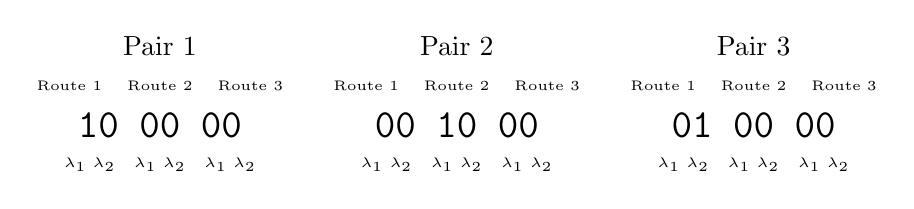
\begin{tikzpicture}[ every node/.style={align=center}]
    % First tuple
    \node at (0,1) {Pair 1};
    \node at (0,0.5) {\tiny Route 1 \quad Route 2 \quad Route 3};
    \node at (0,0) {\Large \texttt{10 00 00}};
    \node at (0,-0.5) {\tiny $\lambda_1 \ \lambda_2 \quad \lambda_1 \ \lambda_2 \quad \lambda_1 \ \lambda_2$};

    % Second tuple
    \node at (3.77,1) {Pair 2};
    \node at (3.77,0.5) {\tiny Route 1 \quad Route 2 \quad Route 3};
    \node at (3.77,0) {\Large \texttt{00 10 00}};
    \node at (3.77,-0.5) {\tiny $\lambda_1 \ \lambda_2 \quad \lambda_1 \ \lambda_2 \quad \lambda_1 \ \lambda_2$};

    % Third tuple
    \node at (7.54,1) {Pair 3};
    \node at (7.54,0.5) {\tiny Route 1 \quad Route 2 \quad Route 3};
    \node at (7.54,0) {\Large \texttt{01 00 00}};
    \node at (7.54,-0.5) {\tiny $\lambda_1 \ \lambda_2 \quad \lambda_1 \ \lambda_2 \quad \lambda_1 \ \lambda_2$};
\end{tikzpicture}
\caption{The bitstring representing a valid solution for an RWA instance where ${P} = 3, N = 3, {\Lambda} = 2$.
	%The bitstring is divided into three sub-bitstrings; each has $3 \times 2$ bits.
	%Each bit represent a selection of unique lightpath the corresponding source-destination pair.
}
\label{fig:bitstring}
\end{figure}

The mixer Hamiltonian that preserves the feasible solution subspace is \begin{align}
	\hat{H}_{m} &= \sum_{i = 1}^{{P}}
	\sum_{j = 1}^{N \times {\Lambda}}
	(\hat{X}_{i,j}\hat{X}_{i, j+1}+\hat{Y}_{i,j}\hat{Y}_{i, j+1}) .
\end{align}
\end{frame}

\begin{frame}{Formulation}{Two-steps scheme}
    \begin{itemize}
\item This amount of qubit may be unpractical when the scheme is applied on a utility scale.
\item The two-steps scheme is as follows:\begin{enumerate}
	\item Reduce the RWA problem into RA problem by letting the number of available wavelength, ${\Lambda} = 1$.
	\item Use the formulation to obtain the route for each source-destination node pair.
	\item Reintroduce the original number of available wavelength and let the route option be the ones obtained from the WA step.
\end{enumerate}
\item The two-step scheme reduces the number of qubits usage from ${P} \times N \times {\Lambda}$ to $\max(
{P} \times N, {P}  \times {\Lambda}
)$.
    
    \end{itemize}
\end{frame}
